\vspace{62mm}
\centering
\section*{\underline{Flugzeugmaße}}

\begin{tikzpicture}[remember picture, overlay]

% ---- ERSTE REIHE: Am Seitenursprung starten
\setlength{\rowheight}{20mm}

    % A1) Erste Kachel unten anbauen
    \setlength{\cellwidth}{35mm}
    \Tile{A1}{([xshift=10mm,yshift=-94mm]current page.north west)}{\cellwidth}{\rowheight}
        {
            \vspace{-\TileSep}
            \titlerm{Flügelstreckung}\\ \vspace{-2mm}
            \begin{equation*}
                \Lambda = \frac{b^2}{S} = \frac{2\,b}{l_\text{i} + l_\text{a}}
            \end{equation*}
        }{0}{1}{1}{0}

    % B1) Zweite Kachel rechts anbauen
    \setlength{\cellwidth}{35mm}
    \Tile{B1}{(A1.north east)}{\cellwidth}{\rowheight}
        {
            \vspace{-\TileSep}
            \titlerm{Neutralpunkt}\\ \vspace{-2mm}
            \begin{equation*}
                x = \frac{l_\mu}{4}
            \end{equation*}
        }{0}{1}{1}{0}

    % C1) Dritte Kachel rechts anbauen
    \setlength{\cellwidth}{28mm}
    \Tile{C1}{(B1.north east)}{\cellwidth}{\rowheight}
        {
            \vspace{-\TileSep}
            \titlerm{Zuspitzung}\\ \vspace{-2mm}
            \begin{equation*}
                \lambda = \frac{l_\text{a}}{l_\text{i}}
            \end{equation*}
        }{0}{1}{1}{0}
    
    % D1) Vierte Kachel rechts anbauen
    \setlength{\cellwidth}{46mm}
    \Tile{D1}{(C1.north east)}{\cellwidth}{\rowheight}
        {
            \vspace{-\TileSep}
            \titlerm{Bezugsflügeltiefe}\\ \vspace{-2mm}
            \begin{equation*}
                l_\mu = \frac{2}{3}\,\frac{1+\lambda+\lambda^2}{1+\lambda}\,l_\text{i}
            \end{equation*}
        }{0}{1}{1}{0}

    % E1) Vierte Kachel rechts anbauen
    \setlength{\cellwidth}{46mm}
    \Tile{E1}{(D1.north east)}{\cellwidth}{\rowheight}
        {
            \vspace{-\TileSep}
            \titlerm{Trapezflügelfläche}\\ \vspace{-2mm}
            \begin{equation*}
                S = \frac{l_\text{i} + l_\text{a}}{2}\,b
            \end{equation*}
        }{0}{0}{1}{0}

% ---- ZWEITE REIHE: unten anbauen
\setlength{\rowheight}{60mm}

    % A2) Erste Kachel unten anbauen
    \setlength{\cellwidth}{64mm}
    \Tile{A2}{(A1.south west)}{\cellwidth}{\rowheight}
        {
            \centering
            \vspace{0.8mm}
            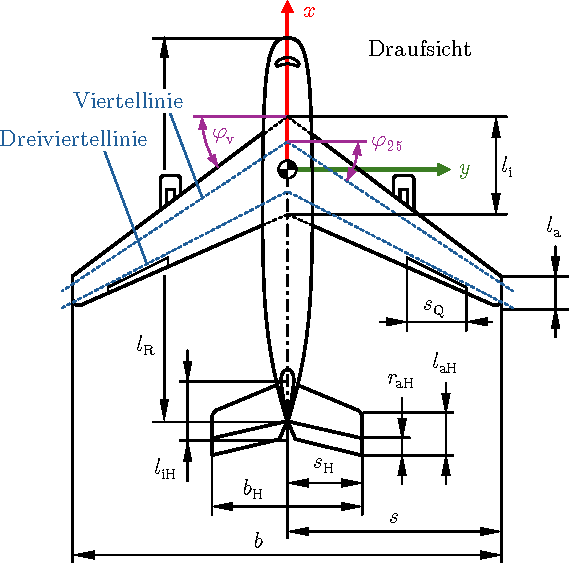
\includegraphics[height=\rowheight-3\TileSep]{images/flugzeug-draufsicht.pdf}
        }{0}{1}{1}{0}

    % B2) Zweite Kachel rechts anbauen
    \setlength{\cellwidth}{44mm}
    \Tile{B2}{(A2.north east)}{\cellwidth}{\rowheight}
        {
            \titlerm{Auftriebsgradient}\\ \vspace{-2mm}
            \begin{equation*}
                \frac{\text{d}C_\text{A}}{\text{d}\alpha} = C_\text{A}' = \frac{2\,\pi\,\Lambda}{\Lambda + 3}
            \end{equation*}
            \resizebox{\cellwidth-2\TileSep}{!}{
            \begin{tabular}{|l|c|} \hline
                Flugzeug-Typ      & $C_\text{A}'$ \\ \hline \hline
                Segelflugzeug     & 25 - 30       \\ \hline
                Transportflugzeug & 7 - 10        \\ \hline
                Reiseflugzeug     & 5 - 7         \\ \hline
                Kampfflugzeug     & 2 - 4         \\ \hline
            \end{tabular}
            }\\ \vspace{4mm}
            \titlerm{Effektive Streckung}\\ \vspace{-2mm}
            \begin{equation*}
                \Lambda\,e
            \end{equation*}
        }{0}{1}{1}{0}

    % C2) Dritte Kachel rechts anbauen
    \setlength{\cellwidth}{82mm}
    \Tile{C2}{(B2.north east)}{\cellwidth}{\rowheight}
        {
            \titlerm{Widerstandsbeiwert}\\ \vspace{-4mm}
            \begin{equation*}
                C_\text{W} = C_\text{W0} + \underbrace{k_\text{p}\,C_\text{A}^2}_\text{Form} + \underbrace{\frac{C_\text{A}^2}{\pi\,\Lambda}\,\left(1+\delta\right)}_\text{Induziert} = C_\text{W0} + \frac{C_\text{A}^2}{\pi\,\Lambda\,e}
            \end{equation*}
            \begin{equation*}
                e = \frac{1}{1+\delta+k_\text{p}\,\pi\,\Lambda} \quad\qquad k_\text{p} = \frac{C_\text{W}-C_\text{W0}}{C_\text{A}^2}
            \end{equation*}%
            \vspace{-1mm}
            \rule{\dimexpr\cellwidth-2\TileSep}{0.5pt} \\ \vspace{0.5mm}
            \titlerm{Abstand Bezugsflügeltiefe}\\ \vspace{-2mm}
            \begin{equation*}
                y_\mu = \frac{b}{6}\,\frac{1+2\,\lambda}{1+\lambda} = \underbrace{\frac{y_{\mu 1}\,S_1 + y_{\mu 2}\,S_2}{S_1 + S_2}}_\text{bei Teilflügeln}
            \end{equation*}
        }{0}{0}{1}{0}

% ---- DRITTE REIHE: unten anbauen
\setlength{\rowheight}{90mm}

    % A3) Erste Kachel unten anbauen
    \setlength{\cellwidth}{120mm}
    \Tile{A3}{(A2.south west)}{\cellwidth}{\rowheight}
        {
            \titlebf{Profilpolaren-Diagramm}\\ \vspace{2mm}
            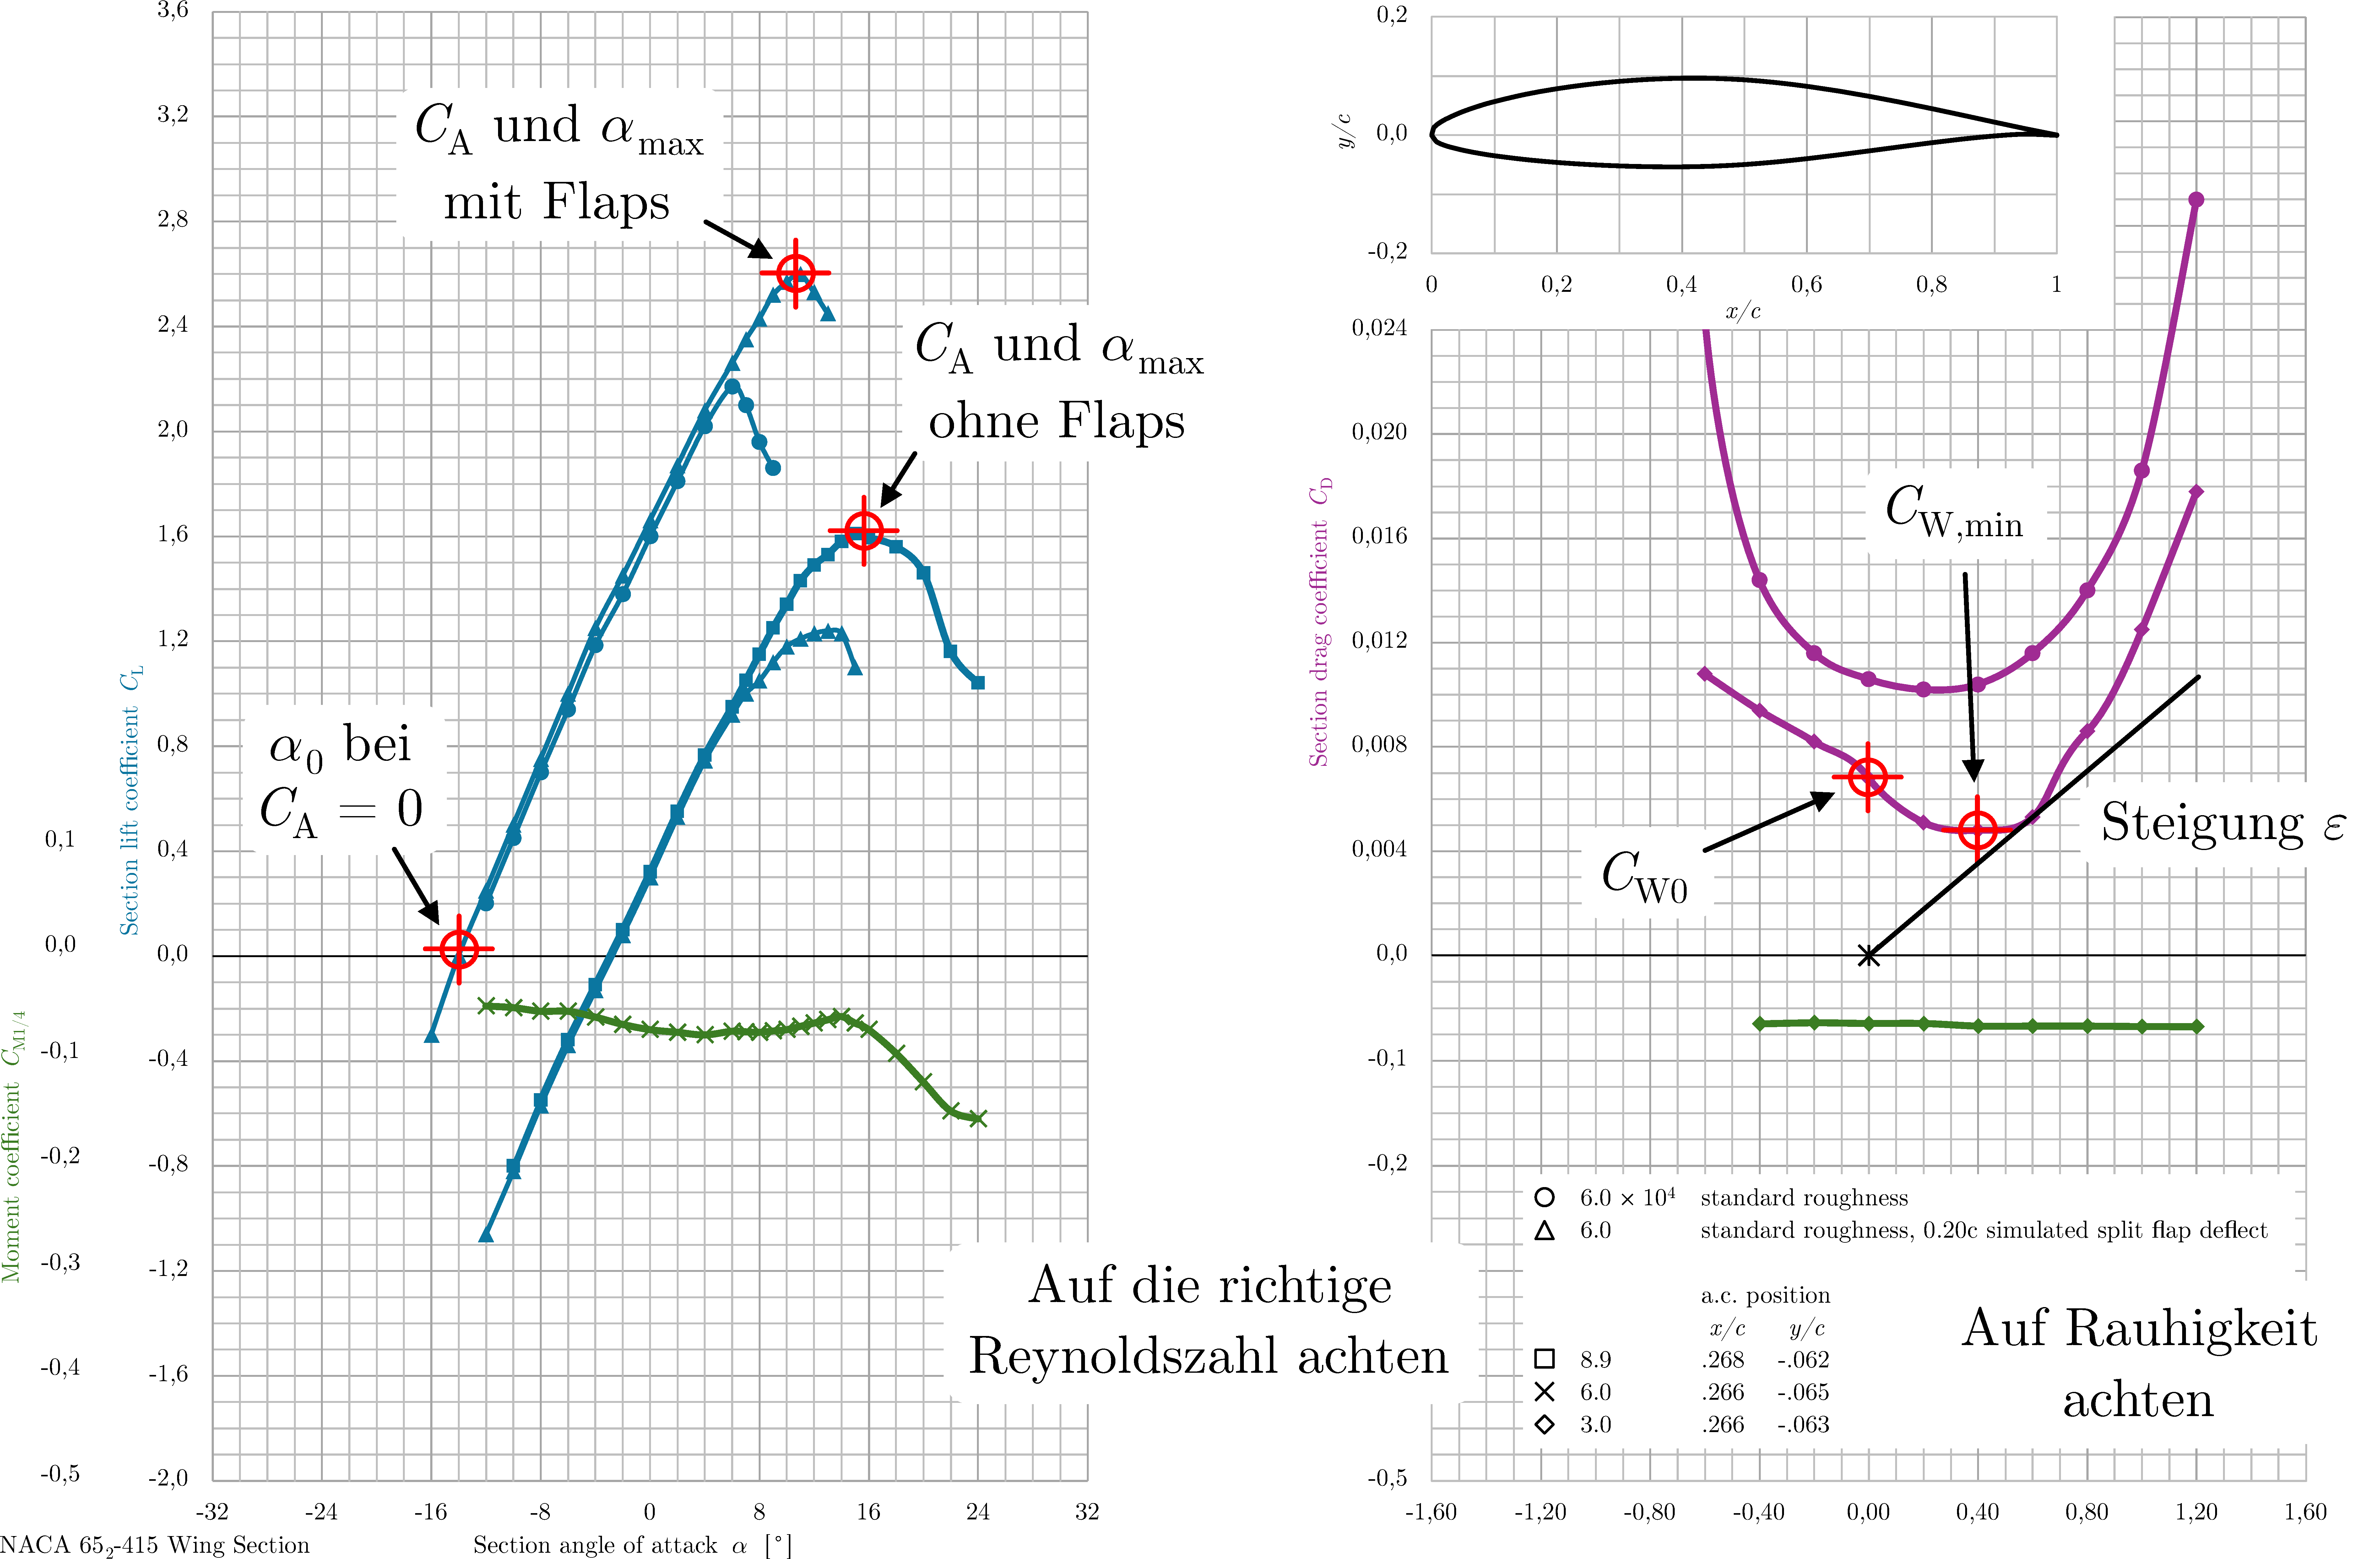
\includegraphics[width=\cellwidth-2\TileSep]{images/profilpolaren-diagramm.pdf}
        }{0}{1}{0}{0}

    % B3) Zweite Kachel rechts anbauen
    \setlength{\cellwidth}{70mm}
    \Tile{B3}{(A3.north east)}{\cellwidth}{\rowheight}
        {
            \titlerm{Nullauftriebsbeiwert}\\ \vspace{-3mm}
            \begin{equation*}
                C_\text{A0} = C_\text{A}\!\left(\alpha=0\right)
            \end{equation*}
            \vspace{-5mm}
            \rule{\dimexpr\cellwidth-2\TileSep}{0.5pt} \\ \vspace{0.5mm}
            \titlerm{Nullwiderstandsbeiwert}\\ \vspace{-3mm}
            \begin{equation*}
                C_\text{W0} = C_\text{W}\!\left(C_\text{A}=0\right)
            \end{equation*}
            \vspace{-5mm}
            \rule{\dimexpr\cellwidth-2\TileSep}{0.5pt} \\ \vspace{2mm}
            \titlebf{Flügelprofil}\\ \vspace{3mm}
            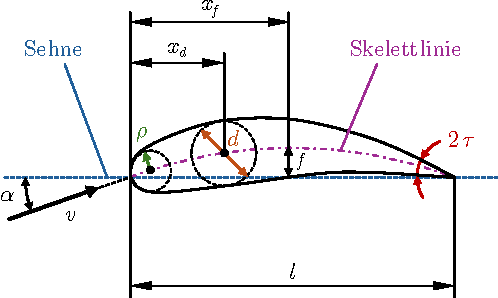
\includegraphics[width=\cellwidth-4\TileSep]{images/profil.pdf}
        }{0}{0}{0}{0}

\end{tikzpicture}

\newpage

\centering
\section*{\underline{Flugzeugmaße}}

\begin{tikzpicture}[remember picture, overlay]

    % ---- VIERTE REIHE: Am Seitenursprung starten
    \setlength{\rowheight}{44mm}

        % X1) EIGENEs FELD für Zeilenüberschrift
        \Tile{X1}{([xshift=10mm,yshift=-16mm]current page.north west)}{190mm}{8mm}
            {
                \titlebf{NACA-Profile}\\
            }{0}{0}{0}{0}

        % A1) Erste Kachel unten anbauen
        \setlength{\cellwidth}{58mm}
        \Tile{A1}{(X1.south west)}{\cellwidth}{\rowheight}
            {
                \vspace{-\TileSep}
                \titlerm{4-Stellig}\\ \vspace{4mm}
                NACA A B CD\\ \vspace{2mm}
                \footnotesize
                \begin{itemize} \setstretch{0.9}
                    \item[A:] Wölbung [\%]
                    \item[B:] Wölbungsrücklage [10\,\% der Tiefe]
                    \item[CD:] Relative Dicke [\%] (= $\delta$)
                \end{itemize}\vspace{2mm}

                Dickenrücklage: immer 30\,\%
            }{0}{1}{1}{0}

        % B1) Erste Kachel rechts anbauen
        \setlength{\cellwidth}{63mm}
        \Tile{B1}{(A1.north east)}{\cellwidth}{\rowheight}
            {
                \vspace{-\TileSep}
                \titlerm{5-Stellig}\\ \vspace{4mm}
                NACA A B C DE\\ \vspace{2mm}
                \footnotesize
                \begin{itemize} \setstretch{0.9}
                    \item[A:] Entwurfs-Auftriebsbeiwert [$\cdot\,0,15$]
                    \item[B:] $\sfrac{1}{5}$ Wölbungsrücklage [10\,\% der Tiefe]
                    \item[C:] Skelettlinie (1: WP, 2: kein WP)*
                    \item[DE:] Relative Dicke [\%]
                \end{itemize}
                \vspace{2mm}
                *WP = Wendepunkt in der Skelettlinie
            }{0}{1}{1}{0}

        % C1) Erste Kachel rechts anbauen
        \setlength{\cellwidth}{69mm}
        \Tile{C1}{(B1.north east)}{\cellwidth}{\rowheight}
            {
                \vspace{-\TileSep}
                \titlerm{6-Stellig}\\ \vspace{4mm}
                NACA A B C - D EF G\\ \vspace{2mm}
                \footnotesize
                \begin{itemize} \setstretch{0.9}
                    \item[A:] Serienbezeichnung (= 6)
                    \item[B:] Lage des min. Druckes in 10\,\% der Tiefe
                    \item[C:] Halber Bereich der Laminardelle $\in\pm 0,1\,\text{C}$
                    \item[D:] $10~\cdot$ Entwurfs-Auftriebsbeiwert
                    \item[EF:] Maximale Dicke [\%]
                    \item[G:] $10~\cdot$ Bereich konst. Übergeschwindigkeit
                \end{itemize}
            }{0}{0}{1}{0}

\end{tikzpicture}